% Auto-generated by export_dashboard_networks_latex.py (nx.to_latex_raw)
% coocc_overall_min10 | nodes=34 edges=90
  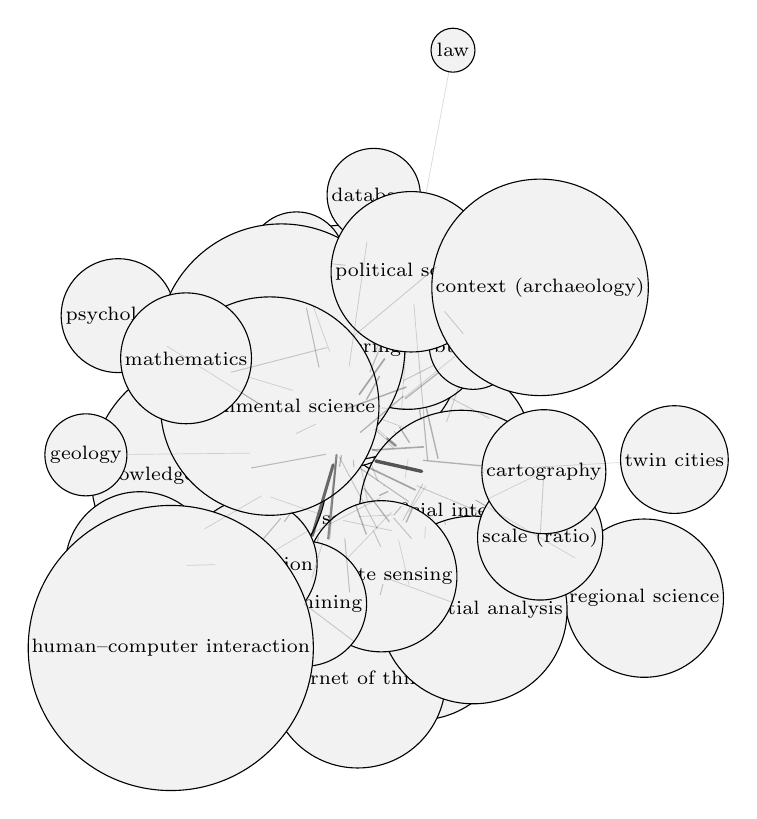
\begin{tikzpicture}[x=1cm,y=1cm,kw/.style={draw,circle,inner sep=1.2pt,font=\scriptsize,fill=black!5},concept/.style={draw,circle,inner sep=1.2pt,font=\scriptsize,fill=blue!10},method/.style={draw,rounded corners=1pt,rectangle,inner sep=1.2pt,font=\scriptsize,fill=orange!12}]
      \draw
        (0.211, -2.115) node[kw] (n0){smart city}
        (0.509, -0.213) node[kw] (n1){urban planning}
        (-0.55, -1.106) node[kw] (n2){computer science}
        (0.618, -1.369) node[kw] (n3){geography}
        (-0.633, -1.938) node[kw] (n4){data science}
        (-0.383, -0.538) node[kw] (n5){engineering}
        (0.91, -1.016) node[kw] (n6){world wide web}
        (-0.437, 0.285) node[kw] (n7){environmental planning}
        (0.346, 0.487) node[kw] (n8){civil engineering}
        (1.029, -1.864) node[kw] (n9){artificial intelligence}
        (-2.173, -1.404) node[kw] (n10){knowledge management}
        (-1.063, 1.332) node[kw] (n11){sociology}
        (-3.328, 0.629) node[kw] (n12){psychology}
        (0.495, -3.354) node[kw] (n13){computer security}
        (-0.285, -4.0) node[kw] (n14){internet of things}
        (3.355, -2.959) node[kw] (n15){regional science}
        (-1.254, 0.225) node[kw] (n16){architectural engineering}
        (-0.082, 2.161) node[kw] (n17){database}
        (1.182, -3.109) node[kw] (n18){geospatial analysis}
        (0.015, -2.681) node[kw] (n19){remote sensing}
        (-3.052, -2.555) node[kw] (n20){3d city models}
        (-0.967, -3.03) node[kw] (n21){data mining}
        (-1.624, -2.524) node[kw] (n22){visualization}
        (2.032, -2.188) node[kw] (n23){scale (ratio)}
        (2.079, -1.353) node[kw] (n24){cartography}
        (3.737, -1.199) node[kw] (n25){twin cities}
        (1.181, 0.25) node[kw] (n26){business}
        (0.395, 1.186) node[kw] (n27){political science}
        (-2.659, -3.592) node[kw] (n28){human–computer interaction}
        (-1.402, -0.52) node[kw] (n29){environmental science}
        (-2.465, 0.087) node[kw] (n30){mathematics}
        (2.031, 0.988) node[kw] (n31){context (archaeology)}
        (-3.737, -1.139) node[kw] (n32){geology}
        (0.925, 4.0) node[kw] (n33){law};
      \begin{scope}[-,line cap=round]
        \draw[line width=0.250pt,opacity=0.150] (n0) to (n1);
        \draw[line width=0.467pt,opacity=0.259] (n0) to (n2);
        \draw[line width=0.322pt,opacity=0.186] (n0) to (n3);
        \draw[line width=0.279pt,opacity=0.164] (n0) to (n4);
        \draw[line width=0.322pt,opacity=0.186] (n0) to (n5);
        \draw[line width=0.264pt,opacity=0.157] (n0) to (n6);
        \draw[line width=0.250pt,opacity=0.150] (n0) to (n13);
        \draw[line width=0.366pt,opacity=0.208] (n0) to (n14);
        \draw[line width=0.467pt,opacity=0.259] (n1) to (n2);
        \draw[line width=0.438pt,opacity=0.244] (n1) to (n3);
        \draw[line width=0.308pt,opacity=0.179] (n1) to (n7);
        \draw[line width=0.496pt,opacity=0.273] (n1) to (n8);
        \draw[line width=0.525pt,opacity=0.288] (n1) to (n5);
        \draw[line width=0.264pt,opacity=0.157] (n1) to (n27);
        \draw[line width=1.250pt,opacity=0.650] (n2) to (n3);
        \draw[line width=0.351pt,opacity=0.201] (n2) to (n7);
        \draw[line width=0.786pt,opacity=0.418] (n2) to (n4);
        \draw[line width=0.511pt,opacity=0.280] (n2) to (n8);
        \draw[line width=1.091pt,opacity=0.570] (n2) to (n5);
        \draw[line width=0.569pt,opacity=0.309] (n2) to (n6);
        \draw[line width=0.598pt,opacity=0.324] (n2) to (n9);
        \draw[line width=0.395pt,opacity=0.222] (n2) to (n10);
        \draw[line width=0.395pt,opacity=0.222] (n2) to (n11);
        \draw[line width=0.250pt,opacity=0.150] (n2) to (n12);
        \draw[line width=0.337pt,opacity=0.193] (n2) to (n16);
        \draw[line width=0.351pt,opacity=0.201] (n2) to (n13);
        \draw[line width=0.366pt,opacity=0.208] (n2) to (n14);
        \draw[line width=0.279pt,opacity=0.164] (n2) to (n17);
        \draw[line width=0.351pt,opacity=0.201] (n2) to (n18);
        \draw[line width=0.482pt,opacity=0.266] (n2) to (n19);
        \draw[line width=0.264pt,opacity=0.157] (n2) to (n20);
        \draw[line width=0.409pt,opacity=0.230] (n2) to (n21);
        \draw[line width=0.409pt,opacity=0.230] (n2) to (n22);
        \draw[line width=0.322pt,opacity=0.186] (n2) to (n23);
        \draw[line width=0.467pt,opacity=0.259] (n2) to (n26);
        \draw[line width=0.482pt,opacity=0.266] (n2) to (n24);
        \draw[line width=0.409pt,opacity=0.230] (n2) to (n27);
        \draw[line width=0.395pt,opacity=0.222] (n2) to (n28);
        \draw[line width=0.409pt,opacity=0.230] (n2) to (n29);
        \draw[line width=0.366pt,opacity=0.208] (n2) to (n30);
        \draw[line width=0.264pt,opacity=0.157] (n2) to (n31);
        \draw[line width=0.250pt,opacity=0.150] (n2) to (n32);
        \draw[line width=0.482pt,opacity=0.266] (n3) to (n7);
        \draw[line width=0.482pt,opacity=0.266] (n3) to (n4);
        \draw[line width=0.453pt,opacity=0.251] (n3) to (n8);
        \draw[line width=0.757pt,opacity=0.404] (n3) to (n5);
        \draw[line width=0.395pt,opacity=0.222] (n3) to (n6);
        \draw[line width=0.250pt,opacity=0.150] (n3) to (n15);
        \draw[line width=0.250pt,opacity=0.150] (n3) to (n16);
        \draw[line width=0.264pt,opacity=0.157] (n3) to (n13);
        \draw[line width=0.337pt,opacity=0.193] (n3) to (n18);
        \draw[line width=0.482pt,opacity=0.266] (n3) to (n19);
        \draw[line width=0.264pt,opacity=0.157] (n3) to (n21);
        \draw[line width=0.279pt,opacity=0.164] (n3) to (n22);
        \draw[line width=0.308pt,opacity=0.179] (n3) to (n23);
        \draw[line width=0.250pt,opacity=0.150] (n3) to (n25);
        \draw[line width=0.308pt,opacity=0.179] (n3) to (n26);
        \draw[line width=0.496pt,opacity=0.273] (n3) to (n24);
        \draw[line width=0.322pt,opacity=0.186] (n3) to (n27);
        \draw[line width=0.366pt,opacity=0.208] (n3) to (n29);
        \draw[line width=0.322pt,opacity=0.186] (n3) to (n9);
        \draw[line width=0.467pt,opacity=0.259] (n4) to (n5);
        \draw[line width=0.293pt,opacity=0.172] (n4) to (n6);
        \draw[line width=0.264pt,opacity=0.157] (n4) to (n9);
        \draw[line width=0.279pt,opacity=0.164] (n4) to (n21);
        \draw[line width=0.250pt,opacity=0.150] (n4) to (n22);
        \draw[line width=0.250pt,opacity=0.150] (n4) to (n10);
        \draw[line width=0.380pt,opacity=0.215] (n5) to (n7);
        \draw[line width=0.598pt,opacity=0.324] (n5) to (n8);
        \draw[line width=0.279pt,opacity=0.164] (n5) to (n6);
        \draw[line width=0.308pt,opacity=0.179] (n5) to (n9);
        \draw[line width=0.279pt,opacity=0.164] (n5) to (n10);
        \draw[line width=0.264pt,opacity=0.157] (n5) to (n11);
        \draw[line width=0.351pt,opacity=0.201] (n5) to (n16);
        \draw[line width=0.337pt,opacity=0.193] (n5) to (n26);
        \draw[line width=0.351pt,opacity=0.201] (n5) to (n27);
        \draw[line width=0.279pt,opacity=0.164] (n5) to (n29);
        \draw[line width=0.293pt,opacity=0.172] (n5) to (n19);
        \draw[line width=0.264pt,opacity=0.157] (n5) to (n30);
        \draw[line width=0.337pt,opacity=0.193] (n7) to (n8);
        \draw[line width=0.293pt,opacity=0.172] (n7) to (n29);
        \draw[line width=0.250pt,opacity=0.150] (n8) to (n27);
        \draw[line width=0.250pt,opacity=0.150] (n9) to (n24);
        \draw[line width=0.322pt,opacity=0.186] (n11) to (n27);
        \draw[line width=0.279pt,opacity=0.164] (n18) to (n19);
        \draw[line width=0.264pt,opacity=0.157] (n20) to (n22);
        \draw[line width=0.322pt,opacity=0.186] (n21) to (n22);
        \draw[line width=0.308pt,opacity=0.179] (n23) to (n24);
        \draw[line width=0.308pt,opacity=0.179] (n26) to (n27);
        \draw[line width=0.250pt,opacity=0.150] (n27) to (n33);
      \end{scope}
    \end{tikzpicture}
